\newcommand{\defaultparindent}{\parindent}
\setlength{\parindent}{0pt}				% \noindent partout
% \parindent in one-column documents is :
% 15pt when the default text size is 10pt,
% 17pt for 11pt,
% and 1.5em for 12pt.
% In two-column documents it is 1em

%\begin{center}
%\begin{tabular}{p{5cm} p{11cm}}
%\textbf{Commandes étudiées :} & \texttt{sh}, \texttt{bash}, \texttt{man}, \texttt{ls}, \texttt{mkdir}, \texttt{touch}, \texttt{chmod}, \texttt{mv}, \texttt{rm}, \texttt{rmdir}, \texttt{cat}, \texttt{file}, \texttt{whereis}, \texttt{which}\\

%\textbf{Builtins étudiées :} & \texttt{pwd}, \texttt{cd}, \texttt{exit}, \texttt{logout}, \texttt{echo}, \texttt{umask}, \texttt{type}, \texttt{>}, \texttt{>{}>}, \texttt{<}, \texttt{<{}<}, \texttt{|}\\

%\textbf{Notions étudiées :} & Tableaux, Pointeurs, Files\\
%\end{tabular}
%\end{center}

\textbf{Notions étudiées :} Tableaux, Pointeurs, Files\\

%\bigskip

\subsection{Rappel sur les files}

\bigskip

Les \textbf{files}, ou \textbf{queues} en anglais, sont des structures visant à stocker et rendre les données dans l'ordre d'arrivée.
Une file dispose donc d'une \textit{tête} contenant l'élément le plus ancien (inséré avant tous les autres), et une \textit{queue} contenant l'élément inséré le plus récemment.
Ces structures sont aussi appelées \textbf{FIFO} (\textit{First In First Out}).\\

\begin{center}
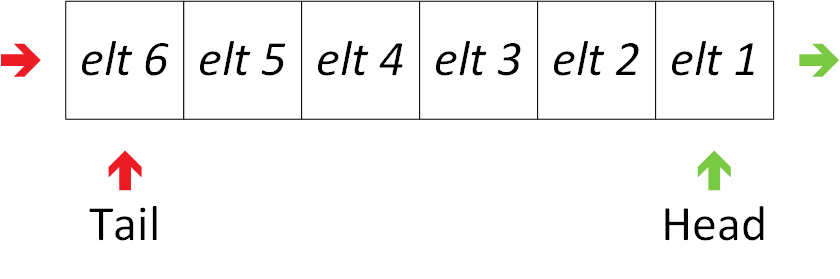
\includegraphics[scale=0.75]{Cours/Files_1_Structure_Generale.png}
\end{center}

\smallskip

Deux opérations permettent d'utiliser une file :
\begin{itemize}
\item \TTBF{ENQUEUE} : permettant d'\textit{enfiler} une donnée supplémentaire dans la file
\item \TTBF{DEQUEUE} : permettant de \textit{défiler} une donnée depuis la file
\end{itemize}
On ajoute donc une donnée en l'enfilant avec un \TTBF{ENQUEUE}, celle-ci se retrouve en \textit{queue} de file, c'est-à-dire au fond de la file.
On récupère une donnée en défilant avec un \TTBF{DEQUEUE}, celle-ci se trouvait en \textit{tête} de file, c'est-à-dire qu'elle attendait son tour depuis son insertion.
On accède donc aux éléments dans l'ordre d'arrivée.\\

Voici un exemple où l'on crée une file, puis on enfile successivement $ 42 $, $ 5 $, et $ 13 $, puis, on défile une fois (pour récupérer $ 42 $), et enfin, on enfile successivement $ 37 $, $ 10 $, $ 24 $, et $ 8 $.\\

\begin{center}
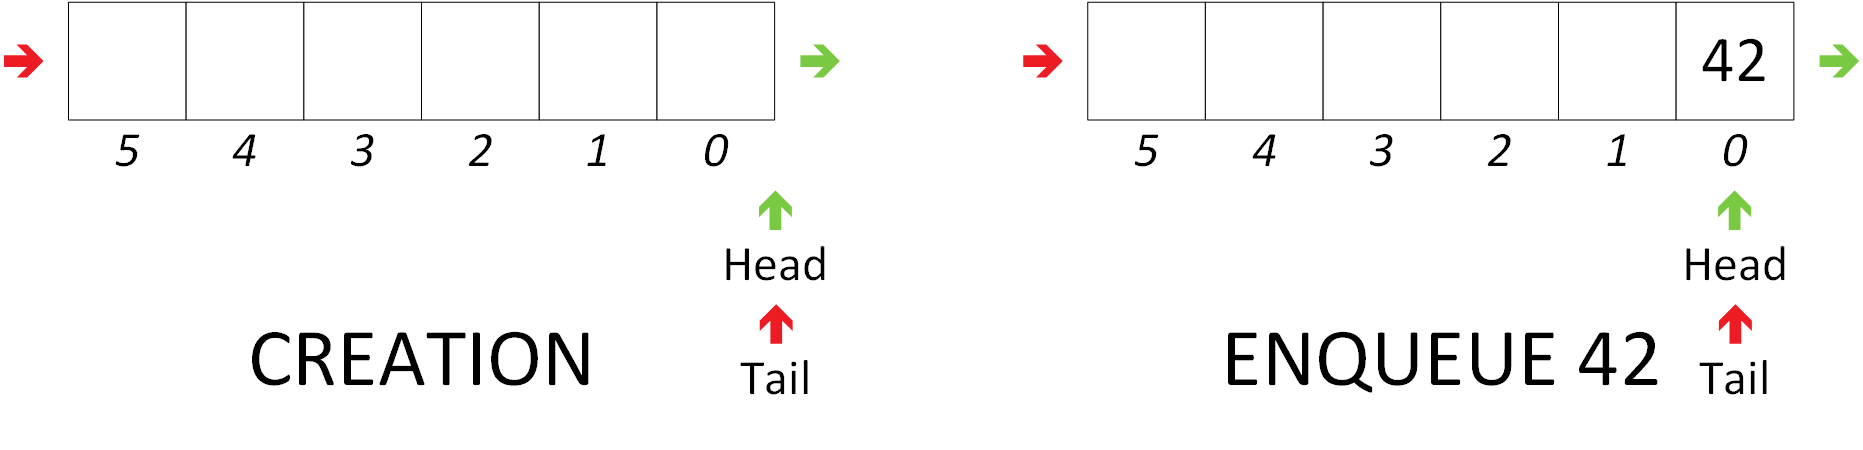
\includegraphics[scale=0.65]{Cours/Files_2_Structure_Generale_Usage_pack_1.png}
\end{center}

\begin{center}
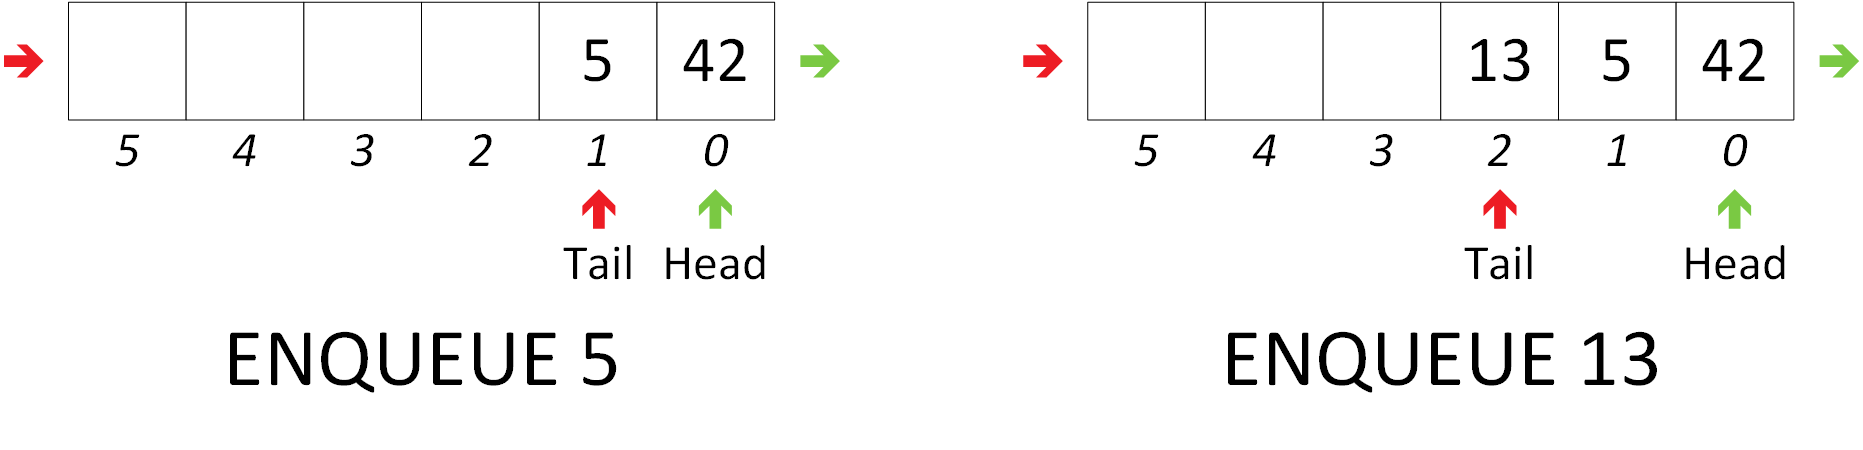
\includegraphics[scale=0.65]{Cours/Files_2_Structure_Generale_Usage_pack_2.png}
\end{center}

\begin{center}
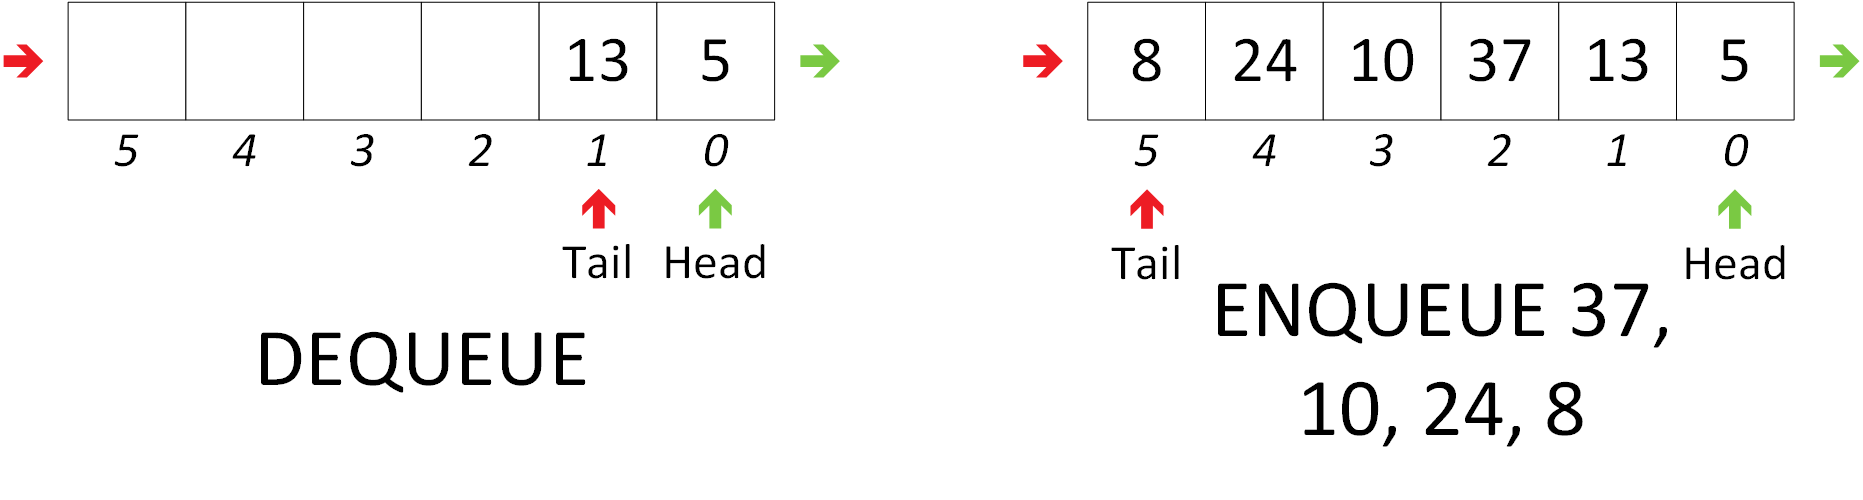
\includegraphics[scale=0.65]{Cours/Files_2_Structure_Generale_Usage_pack_3.png}
\end{center}

\smallskip

Les files, et surtout le respect de l'ordre d'arrivée des objets, sont couramment utilisés : mise en attente de personnes face à des guichets (voitures à un péage, clients face à une caisse, etc).

En informatique, on utilisera les files pour stocker temporairement et traiter les requêtes dans leur ordre d'arrivée.
Dans le cas des \textit{schedulers} (ordonnanceurs) visant à déterminer quel processus exécuter sur le c\oe{}ur d'un processus, on ajoute parfois une priorité à chaque objet de la file.
Ceci implique de mettre à jour l'ordre des objets dans la file lors de certains évènements (par exemple lorsque l'on enfile ou défile un élément, ou après un certain temps).\\

Afin d'implémenter une file, il est donc nécessaire d'avoir un espace de stockage ordonné (un tableau numéroté ou une liste chaînée), et deux indicateurs pour l'élément tête de file et l'élément en queue de file.
Nous allons maintenant voir comment implémenter une file avec des listes chaînées et un tableau de taille fixe.

\bigskip

%%%%%%%%%%%%%%%%%%%%%%%%%%%%%%%%%%%%%%%%%%%%%%%%%%%%%%%%%%%%
%%%%%%%%%%%%%%%%%%%%%%%%%%%%%%%%%%%%%%%%%%%%%%%%%%%%%%%%%%%%
%%%%%%%%%%%%%%%%%%%%%%%%%%%%%%%%%%%%%%%%%%%%%%%%%%%%%%%%%%%%

\subsection{Files : implémentation avec des listes chaînées}

\bigskip

Une implémentation à l'aide d'une liste chaînée permet d'exploiter la mémoire et d'être donc beaucoup plus flexible en terme de nombre maximum d'éléments.
Le schéma suivant illustre une file sous forme de liste chaînée en mémoire :\\

\begin{center}
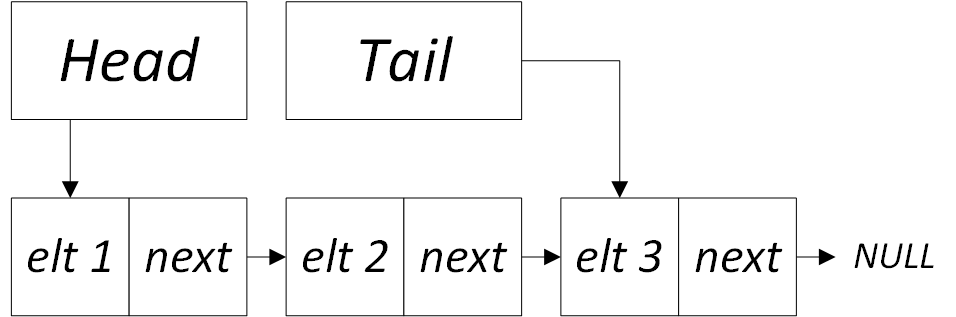
\includegraphics[scale=0.75]{Cours/Files_3_Liste_Chainee_Structure_cas_general.png}
\end{center}

\smallskip

On y retrouve plusieurs fois la structure typique des listes chaînées (un élément et un pointeur vers l'élément suivant), ainsi que deux pointeurs indiquant respectivement la tête de la file (\textit{head}) et la queue de la file (\textit{tail}).

Deux cas particuliers concernent les files où le pointeur de tête et le pointeur de queue valent la même chose : la file vide où les pointeurs contiennent \TTBF{NULL}, et la file contenant un seul élément vers lequel les deux pointeurs renvoient.
Une file nouvellement créée se trouve dans l'état vide.\\

\begin{center}
%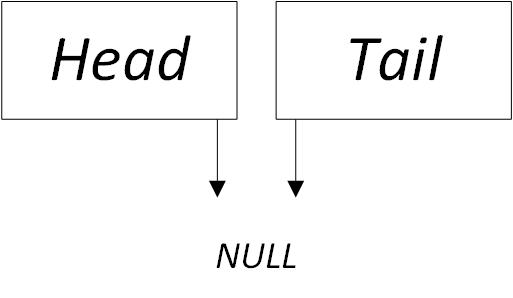
\includegraphics[scale=0.75]{Cours/Files_3_Liste_Chainee_Structure_cas_vide.png}
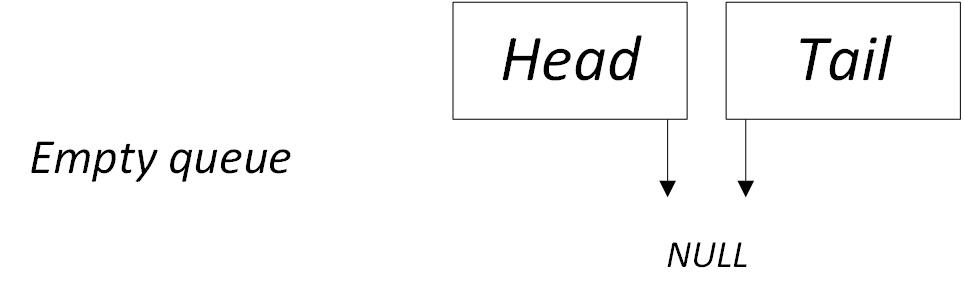
\includegraphics[scale=0.75]{Cours/Files_3_Liste_Chainee_Structure_cas_vide_etiquette.png}
\end{center}

\smallskip

\begin{center}
%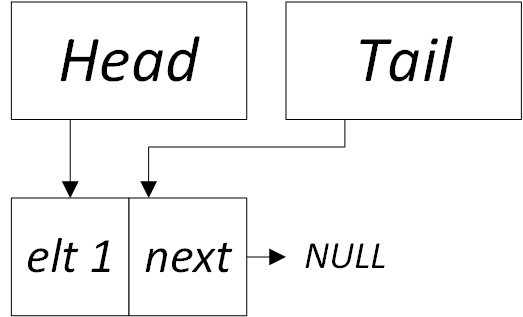
\includegraphics[scale=0.75]{Cours/Files_3_Liste_Chainee_Structure_cas_1_elt.png}
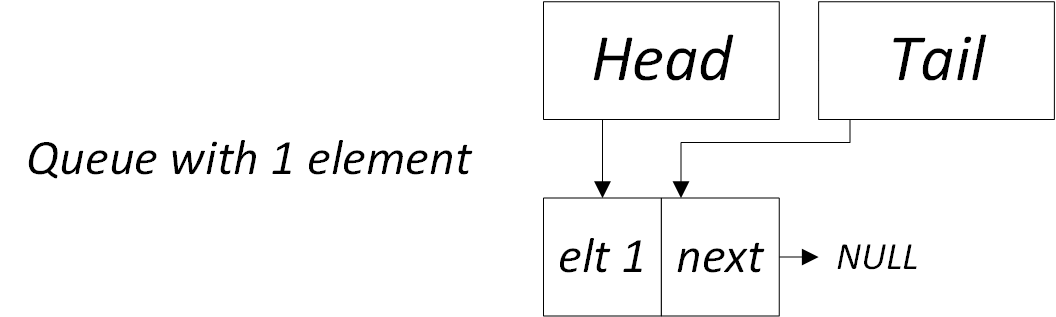
\includegraphics[scale=0.75]{Cours/Files_3_Liste_Chainee_Structure_cas_1_elt_etiquette.png}
\end{center}

\smallskip

L'exemple suivant montre l'évolution d'une file au fur et à mesure des insertions (enfiler / \TTBF{ENQUEUE}) et suppressions (défiler / \TTBF{DEQUEUE}).\\

\begin{center}
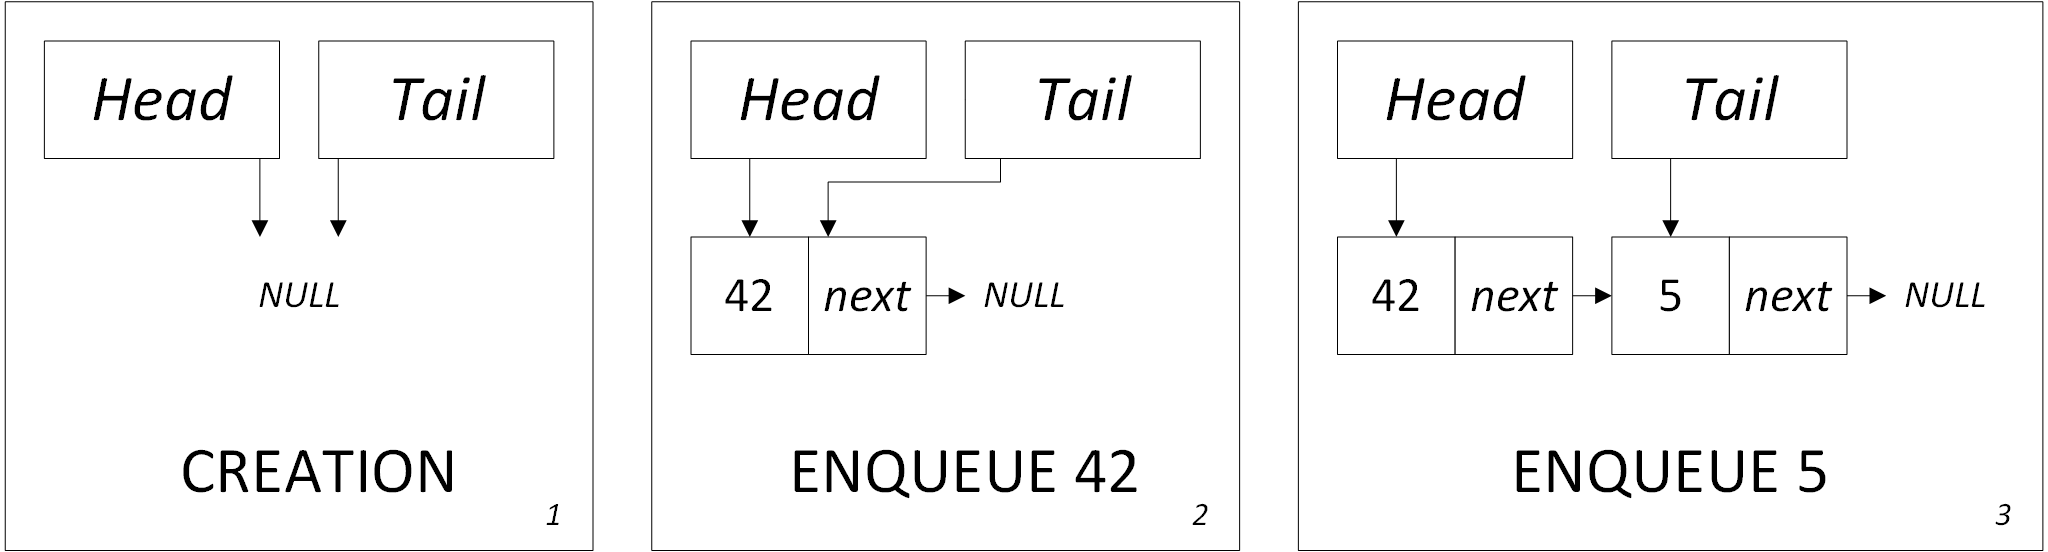
\includegraphics[scale=0.60]{Cours/Files_4_Liste_Chainee_Usage_pack_1.png}
\end{center}

\begin{center}
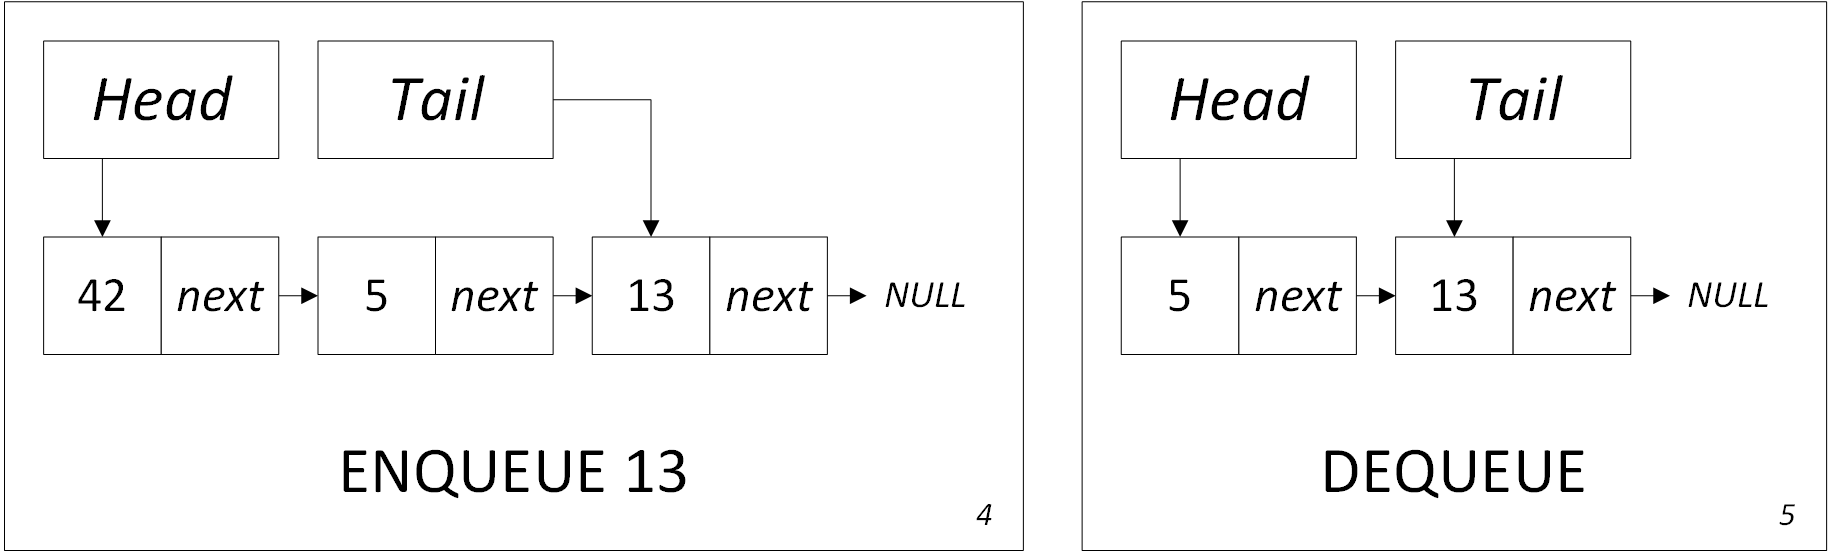
\includegraphics[scale=0.60]{Cours/Files_4_Liste_Chainee_Usage_pack_2.png}
\end{center}

\smallskip

Les principales opérations se résument ainsi :
\begin{itemize}
\item Création : on alloue en mémoire la structure générale de la file, et on fixe les tête et queue de la file à \TTBF{NULL}.
\item Enfiler : on alloue en mémoire un nouvel élément, on met son pointeur \textit{next} à \TTBF{NULL}, puis, si la file est vide, on met les pointeurs de tête et de queue sur le nouvel élément, sinon, on met l'adresse du nouvel élément sur le pointeur \textit{next} de l'élément pointé par la queue, et on met à jour le pointeur de queue sur le nouvel élément.
\item Défiler : si la file est vide, on retourne une erreur, sinon, on récupère tout d'abord l'adresse de l'élément suivant celui en tête, puis, on libère l'élément en tête, puis, on met à jour le pointeur de tête de la file vers l'adresse de l'élément suivant. Si l'élément suivant est \TTBF{NULL}, on met à jour le pointeur de queue également.
\item Vider : on défile successivement tous les éléments jusqu'à obtenir la tête à \TTBF{NULL} (ne pas oublier que l'opération qui défile met à jour la queue dans le cas \TTBF{NULL}).
\item Tête : on renvoie le contenu de l'élément en tête de file (le prochain élément qui sera défilé).
\item Queue : on renvoie le contenu de l'élément en queue de file (le dernier élément qui sera défilé).
\end{itemize}

\bigskip

%%%%%%%%%%%%%%%%%%%%%%%%%%%%%%%%%%%%%%%%%%%%%%%%%%%%%%%%%%%%
%%%%%%%%%%%%%%%%%%%%%%%%%%%%%%%%%%%%%%%%%%%%%%%%%%%%%%%%%%%%
%%%%%%%%%%%%%%%%%%%%%%%%%%%%%%%%%%%%%%%%%%%%%%%%%%%%%%%%%%%%

\subsection{Files : implémentation avec un tableau de taille fixe}

\bigskip

Une implémentation avec un tableau de taille fixe impose cette fois une limitation : la file aura une taille maximale, et on peut refuser l'ajout d'un élément si la file est déjà pleine.
La structure diffère également du fait que le tableau est alloué une seule fois lors de sa création (voire même lors de la compilation dans le cas statique).

Le schéma suivant présente la structure générale :\\

\begin{center}
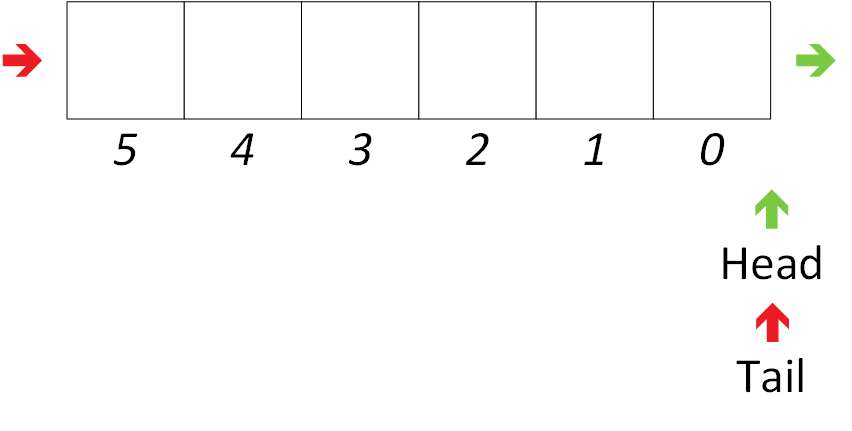
\includegraphics[scale=1]{Cours/Files_5_Tableau_Statique_Structure.png}
\end{center}

\smallskip

On notera cette fois que plusieurs informations distinctes doivent être conservées : l'adresse du tableau, le numéro de case correspondant à la tête de la file (\textit{head}), le numéro de case correspondant à la queue de la file (\textit{tail}), la taille du tableau (le nombre maximum d'objets pouvant être stockés), le nombre d'éléments dans le tableau.

Le schéma suivant détaille certaines informations de façon plus explicite :\\

\begin{center}
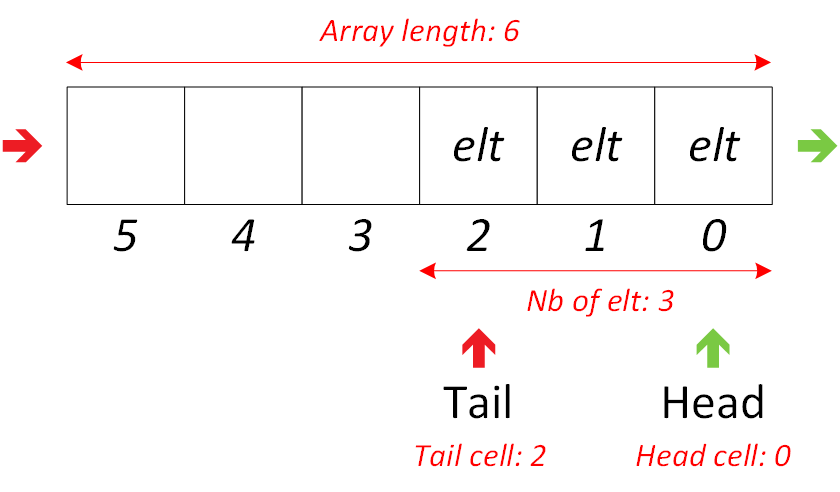
\includegraphics[scale=1]{Cours/Files_5_Tableau_Statique_Structure_Detaillee_1.png}
\end{center}

\smallskip

Une façon d'implémenter le tableau permet de supposer que la case $ 0 $ contiendra toujours l'élément de tête.
Dans ce cas très précis, on peut donc se passer de la variable de tête, et au contraire, s'appuyer sur la variable donnant le nombre d'éléments dans le tableau pour savoir si la file est vide ou non.
Cette implémentation ressemble donc à cela :\\

\begin{center}
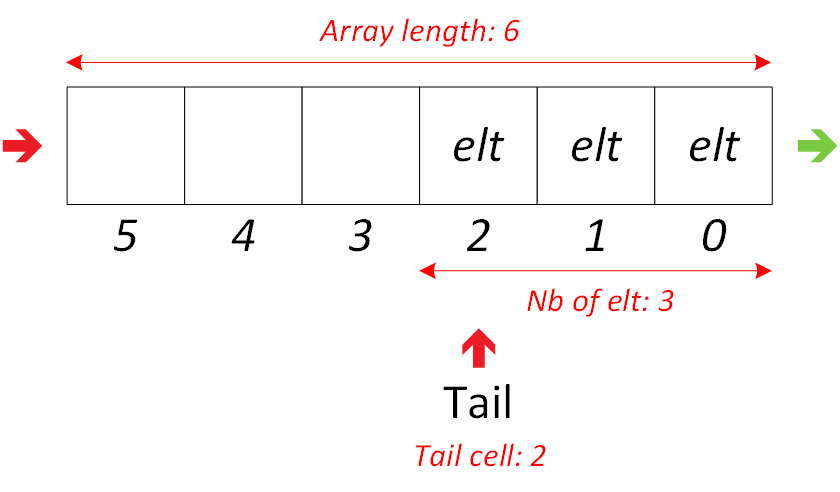
\includegraphics[scale=1]{Cours/Files_5_Tableau_Statique_Structure_Detaillee_2.png}
\end{center}

\smallskip

Dans le cas d'un tableau de taille fixe, les pointeurs de tête et de queue ne peuvent pas utiliser la valeur \TTBF{NULL} comme indicateur de tableau vide, car cette valeur est égale à $ 0 $ (ce qui laisserait à penser que la queue est effectivement à la case 0).
Plusieurs solutions sont possibles pour indiquer les cases où se trouvent la tête et la queue de la file, ainsi que le cas vide :

\begin{itemize}
\item On enregistre dans la structure de la file une variable servant à compter le nombre d'éléments présents (la queue peut donc prendre n'importe quelle valeur tant que la file est vide).
\item On utilise un entier relatif pour indiquer la position, et $ -1 $ indique que la file est vide (l'ajout d'un élément décalera la tête et la queue à $ 0 $, c'est-à-dire la case où sera l'élément).
\item On place la queue de la file sur la première case non utilisée, et l'accès au dernier élément se fait donc en retirant $ 1 $ au pointeur de sommet (ainsi, une queue à la case $ 0 $ indique que la file est vide).
Attention : dans ce cas précis, un tableau plein aura un sommet hors des cases du tableau (il ne faudra donc \textit{jamais} le déréférencer s'il atteinte une telle valeur).
\item On représente complètement différemment la file : on décale les pointeurs de tête et de queue au fur et à mesure des insertions et suppressions ($ +1 $ / $ -1 $). Le pointeur de queue peut passer de la dernière case à la première, car les éléments actuellement dans la file se trouvent uniquement entre la tête et la queue.
Vider ce tableau revient uniquement à passer les pointeurs à la valeur $ -1 $.
Attention : dans ce cas précis, il est nécessaire de faire très attention à l'ordre de lecture des éléments entre la tête et la queue.
\end{itemize}

\smallskip

L'exemple suivant montre l'évolution d'une file implémentée avec un tableau fixe au fur et à mesure des ajouts (enfiler / \TTBF{ENQUEUE}) et suppressions (défiler / \TTBF{DEQUEUE}).\\

\begin{center}
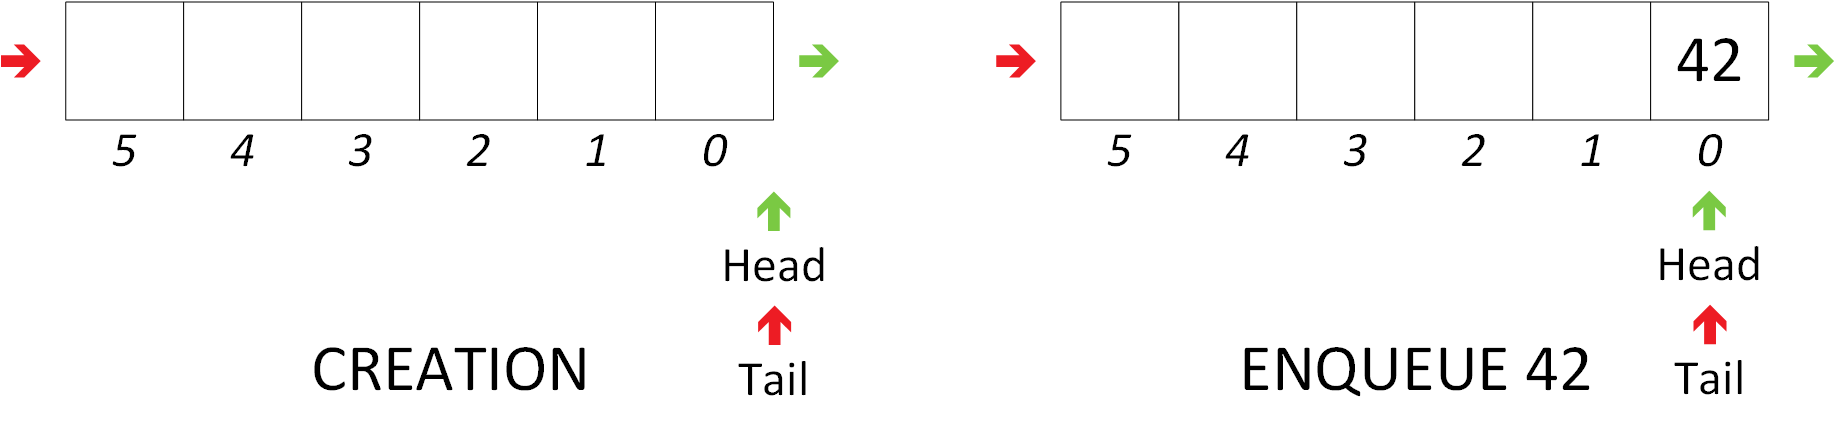
\includegraphics[scale=0.65]{Cours/Files_6_Tableau_Statique_Usage_pack_1.png}
\end{center}

\begin{center}
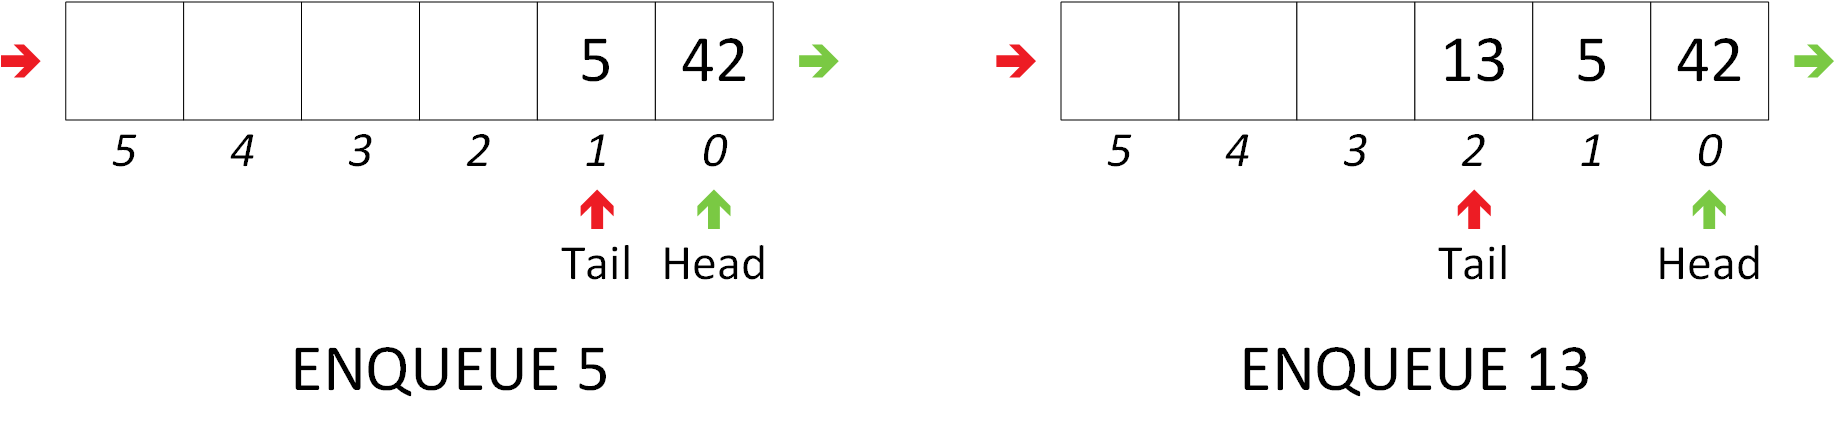
\includegraphics[scale=0.65]{Cours/Files_6_Tableau_Statique_Usage_pack_2.png}
\end{center}

\smallskip

Dans les schémas suivants, deux versions sont présentées :
\begin{itemize}
\item celui de gauche présente la version standard où la tête ne bouge pas (il est nécessaire de décaler l'ensemble des éléments du tableau dès que l'on défile),
\item celui de droite présente la version où seuls les pointeurs de tête et de queue sont décalés (il faut faire attention à l'ordre de lecture entre la tête et la file, et s'appuyer sur les modulos).
\end{itemize}

\begin{center}
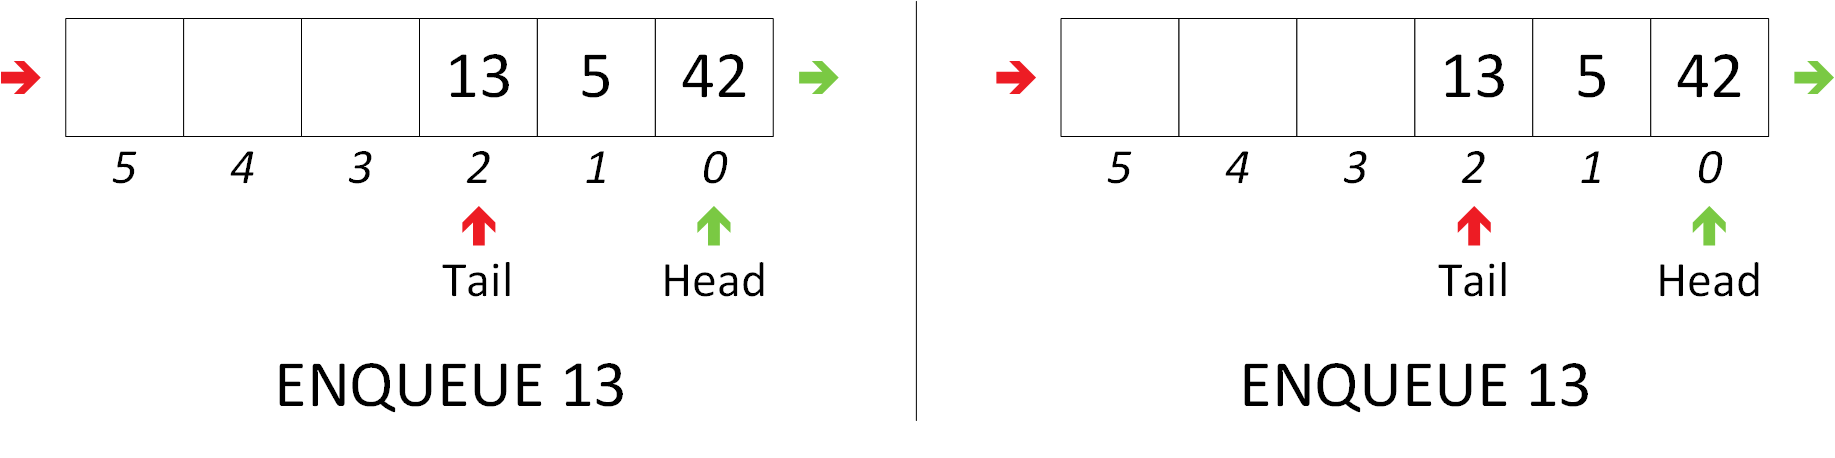
\includegraphics[scale=0.65]{Cours/Files_6_Tableau_Statique_Usage_pack_2_double.png}
\end{center}

\begin{center}
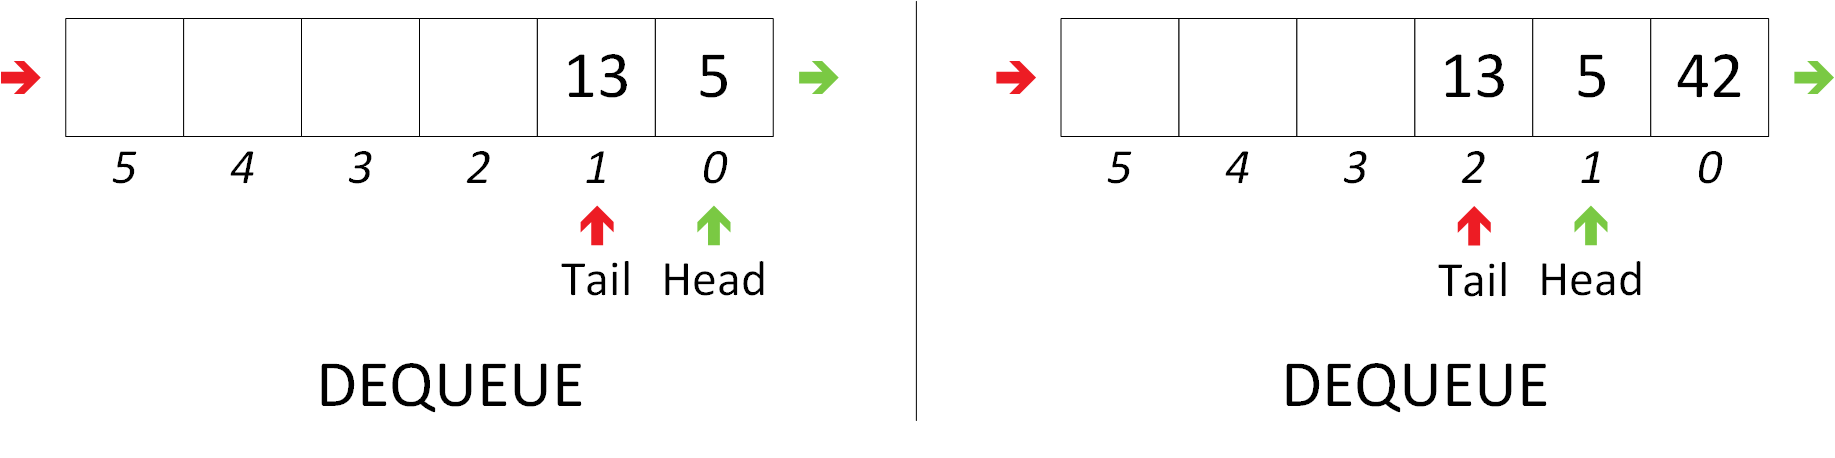
\includegraphics[scale=0.65]{Cours/Files_6_Tableau_Statique_Usage_pack_3.png}
\end{center}

\begin{center}
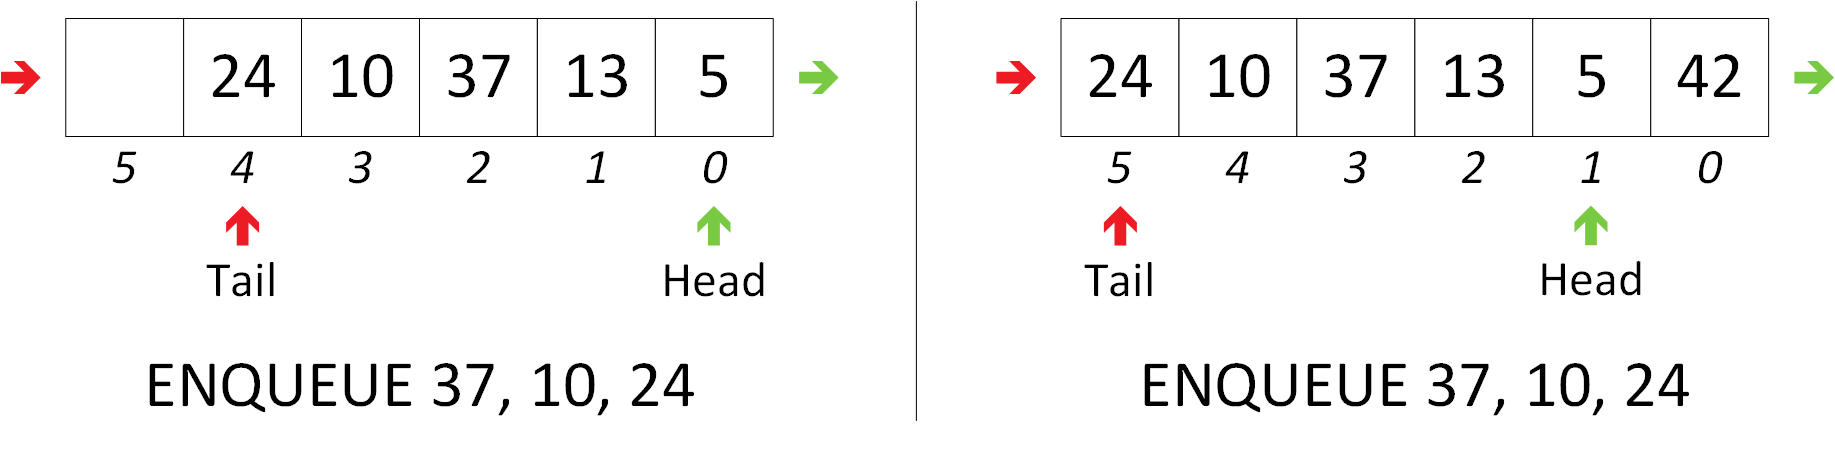
\includegraphics[scale=0.65]{Cours/Files_6_Tableau_Statique_Usage_pack_4.png}
\end{center}

\begin{center}
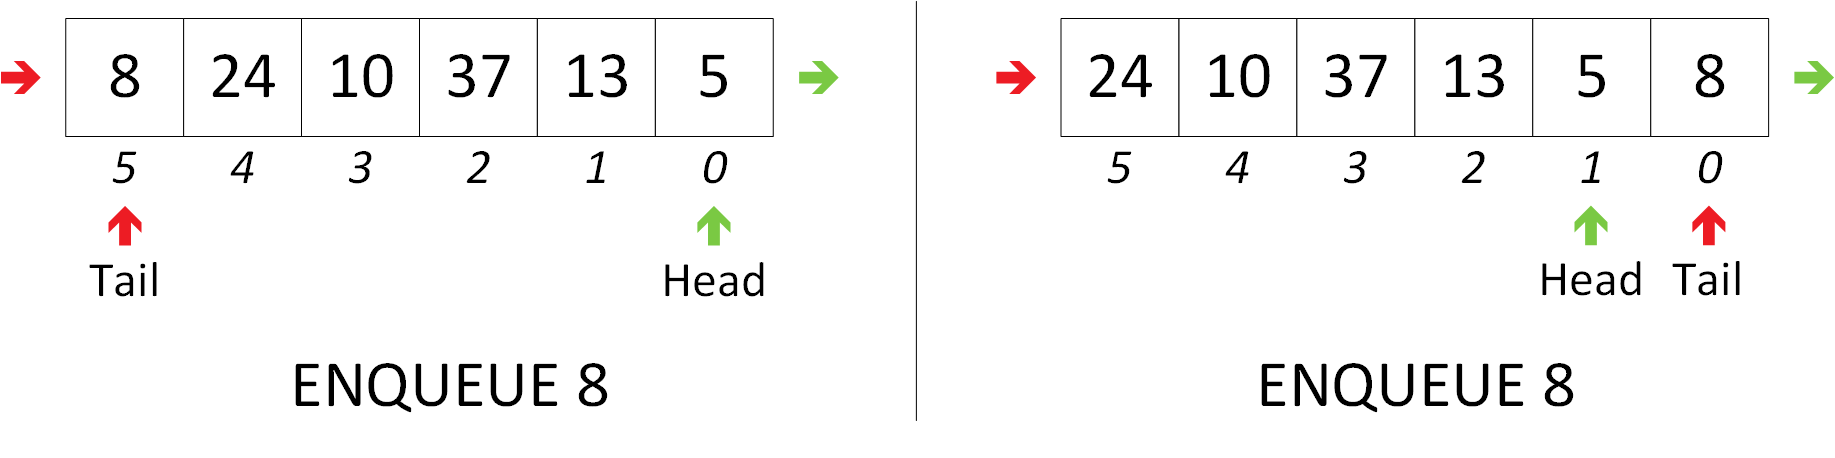
\includegraphics[scale=0.65]{Cours/Files_6_Tableau_Statique_Usage_pack_5.png}
\end{center}

\smallskip

Dans ce dernier cas, lorsque le tableau de gauche était complètement rempli, on a décalé le pointeur de queue au début du tableau, simplement en utilisant un modulo de la taille du tableau.
Il est important de respecter l'ordre de lecture : on lit bel et bien depuis le pointeur de tête, en effectuant un $ +1 $ (lecture vers la gauche) tout en appliquant un modulo de la taille du tableau au résultat, jusqu'à atteindre le pointeur de queue.

On peut également comprendre qu'il y a eu un dépassement en comparant la position du pointeur de tête et de queue : la différence entre leurs positions est négative ! \linebreak
($ pos. tail - pos. head = 0 - 1 = -1$)

\bigskip

Cette autre façon de gérer la file est un tout petit peu plus complexe dans l'écriture des algorithmes de gestion, mais elle évite énormément de réécritures dans le tableau/en mémoire (inutile de lire une case, l'écrire ailleurs, et recommencer ainsi de suite lors de chaque \textit{dequeue}).
Pour ce TP, vous êtes libres de choisir l'implémentation que vous souhaitez réaliser.

\bigskip

Les principales opérations se résument ainsi :
\begin{itemize}
\item Création : on alloue en mémoire le tableau (sauf s'il est statique), et on fixe la tête et la queue de la file à la valeur prévue pour démarrer ($ -1 $, $ 0 $, ou toute autre valeur choisie) [éventuellement, on met à jour le nombre d'objets dans le tableau en le fixant à $ 0 $].
\item Enfiler : si le tableau est plein, on retourne une erreur, sinon, on ajoute le nouvel élément à gauche de la position du pointeur de queue, et on décale la queue de la file d'un cran à gauche [éventuellement, on met à jour le nombre d'objets dans le tableau].
Autre version : on ajoute le nouvel élément dans la case à gauche de la position du pointeur de queue modulo la taille du tableau, et on décale la queue de la file.
\item Défiler : si la file est vide, on retourne une erreur, sinon, on décale l'ensemble des éléments vers la droite [éventuellement, on met à jour le nombre d'objets dans le tableau].
Autre version : on décale la tête de la file d'un cran à gauche.
\item Vider : on fixe les pointeurs de tête et de queue à la valeur prévue pour démarrer ($ -1 $, $ 0 $, ou toute autre valeur choisie) [éventuellement, on met à jour le nombre d'objets dans le tableau en le fixant à $ 0 $].
\item Tête : on renvoie le contenu de la case du pointeur de tête de file (le prochain élément qui sera défilé).
\item Queue : on renvoie le contenu de la case du pointeur de queue de file (le dernier élément qui sera défilé).
\end{itemize}

\setlength{\parindent}{\defaultparindent}
